\chapter{Supplementary Material to Chapter~\ref{chp:con} - Coupled Oscillator Networks
% - ISS Coupled Oscillator Networks for Closed-form Model-based Control in Latent Space 
}\label{chp:apx:con}

\textit{
% This appendix contains supplementary material for Chapter~\ref{chp:con}. Specifically, we report additional details on the training and evaluation process, such as the reporting of the mathematical definition of all considered baseline methods and evaluation metrics, additional results for learning latent dynamics, such as a complete set of evaluation metrics and number of trainable parameters for all evaluated methods, and sequences of stills of the prediction results of \gls{CON} on all datasets, and additional results for the model-based latent space control, including the baselines of a pure feedback controller based on a \gls{NODE} model, and a pure feedback controller based on the learned \gls{CON} dynamics.
\noindent This appendix provides supplementary material for Chapter~\ref{chp:con}. In particular, we offer further details on the training and evaluation process, including the mathematical definitions of all baseline methods and evaluation metrics considered. Additionally, we present extra results on learning latent dynamics—such as a complete set of evaluation metrics and the number of trainable parameters for every evaluated method—as well as sequences of stills illustrating the prediction results of \gls{CON} across all datasets. Finally, we include additional findings on model-based latent space control, featuring baselines like a pure feedback controller based on a \gls{NODE} model and one based on the learned \gls{CON} dynamics.
}

\blfootnote{
    This appendix is partly based on \faFileTextO \, \faTrophy~\emph{\textbf{M. Stölzle}, and C. Della Santina (2024). Input-to-State Stable Coupled Oscillator Networks for Closed-form Model-based Control in Latent Space. In Proceedings of Advances in Neural Information Processing Systems (NeurIPS) 37, \textbf{Spotlight}~\citep{stolzle2024input}.}
    M.S. and C.D.S conceived the project, developed the formulation of the coupled oscillator network, and derived the stability proof.
    M.S. devised the closed-form approximation to the \gls{CON} dynamics, came up with the model-based control approach, and implemented the training and control pipeline.
    M.S. planned and conducted all experiments and wrote the manuscript.
    C.D.S. revised the manuscript, provided funding, and supervised the project.
}

\newpage

\section{Appendix on experimental setup and datasets}\label{sec:apx-con:experimental_setup}

\subsection{Autoencoder architecture}
For the encoder and decoder, we rely on a vanilla \glspl{CNN} implemented as a $\beta$-\gls{VAE}~\cite{kingma2014auto}.

\textbf{Encoder.} The encoder consists of two convolutional layers with kernel size $(3, 3)$ and stride $(1, 1)$ mapping to $16$, $32$, respectively.
The features are flattened and then passed to two linear layers with hidden dimension $256$ and $n_z$.
Each layer (except for the last) is followed by a layer norm~\cite{ba2016layer} and a LeakyReLU nonlinearity.

\textbf{Decoder.} The decoder first uses two linear layers to map to hidden dimensions of $256$ and $32768$, respectively.
We then apply two 2D transposed convolutions~\cite{dumoulin2016guide} reducing the number of channels first to $16$, and then to $1$.
Each layer (except for the last linear and last convolutional) is followed by a layer norm~\cite{ba2016layer} and a LeakyReLU nonlinearity.
Finally, we apply a sigmoid function to clip the output into the range $[-1, 1]$.

\subsection{Latent dynamic models}\label{sub:apx-con:latent_dynamic_models}
In the following section, we provide implementation details for the latent dynamic models that we evaluated as part of this work.

\subsubsection{Coupled Oscillator Network (CON)}\label{ssub:apx-con:latent_space_dynamic_models:con}
We leverage the \gls{CON} in $\mathcal{W}$-coordinates given by \eqref{eq:con:conw_dynamics} for learning latent space dynamics. 
Specifically, we consider the input-to-force mapping $g(u)) = B(u) \, u(t)$, where $B(u) \in \mathbb{R}^{n \times m}$ is parametrized by few-layer \gls{MLP}. We report results for two different sizes of the \gls{MLP}: one medium-sized variant consisting of five layers with a hidden dimension of $30$ and a small variant with two layers and a hidden dimension of $12$. In both cases, we use a hyperbolic tangent as a nonlinearity.


% \begin{figure}[hbt]
%     \centering
%     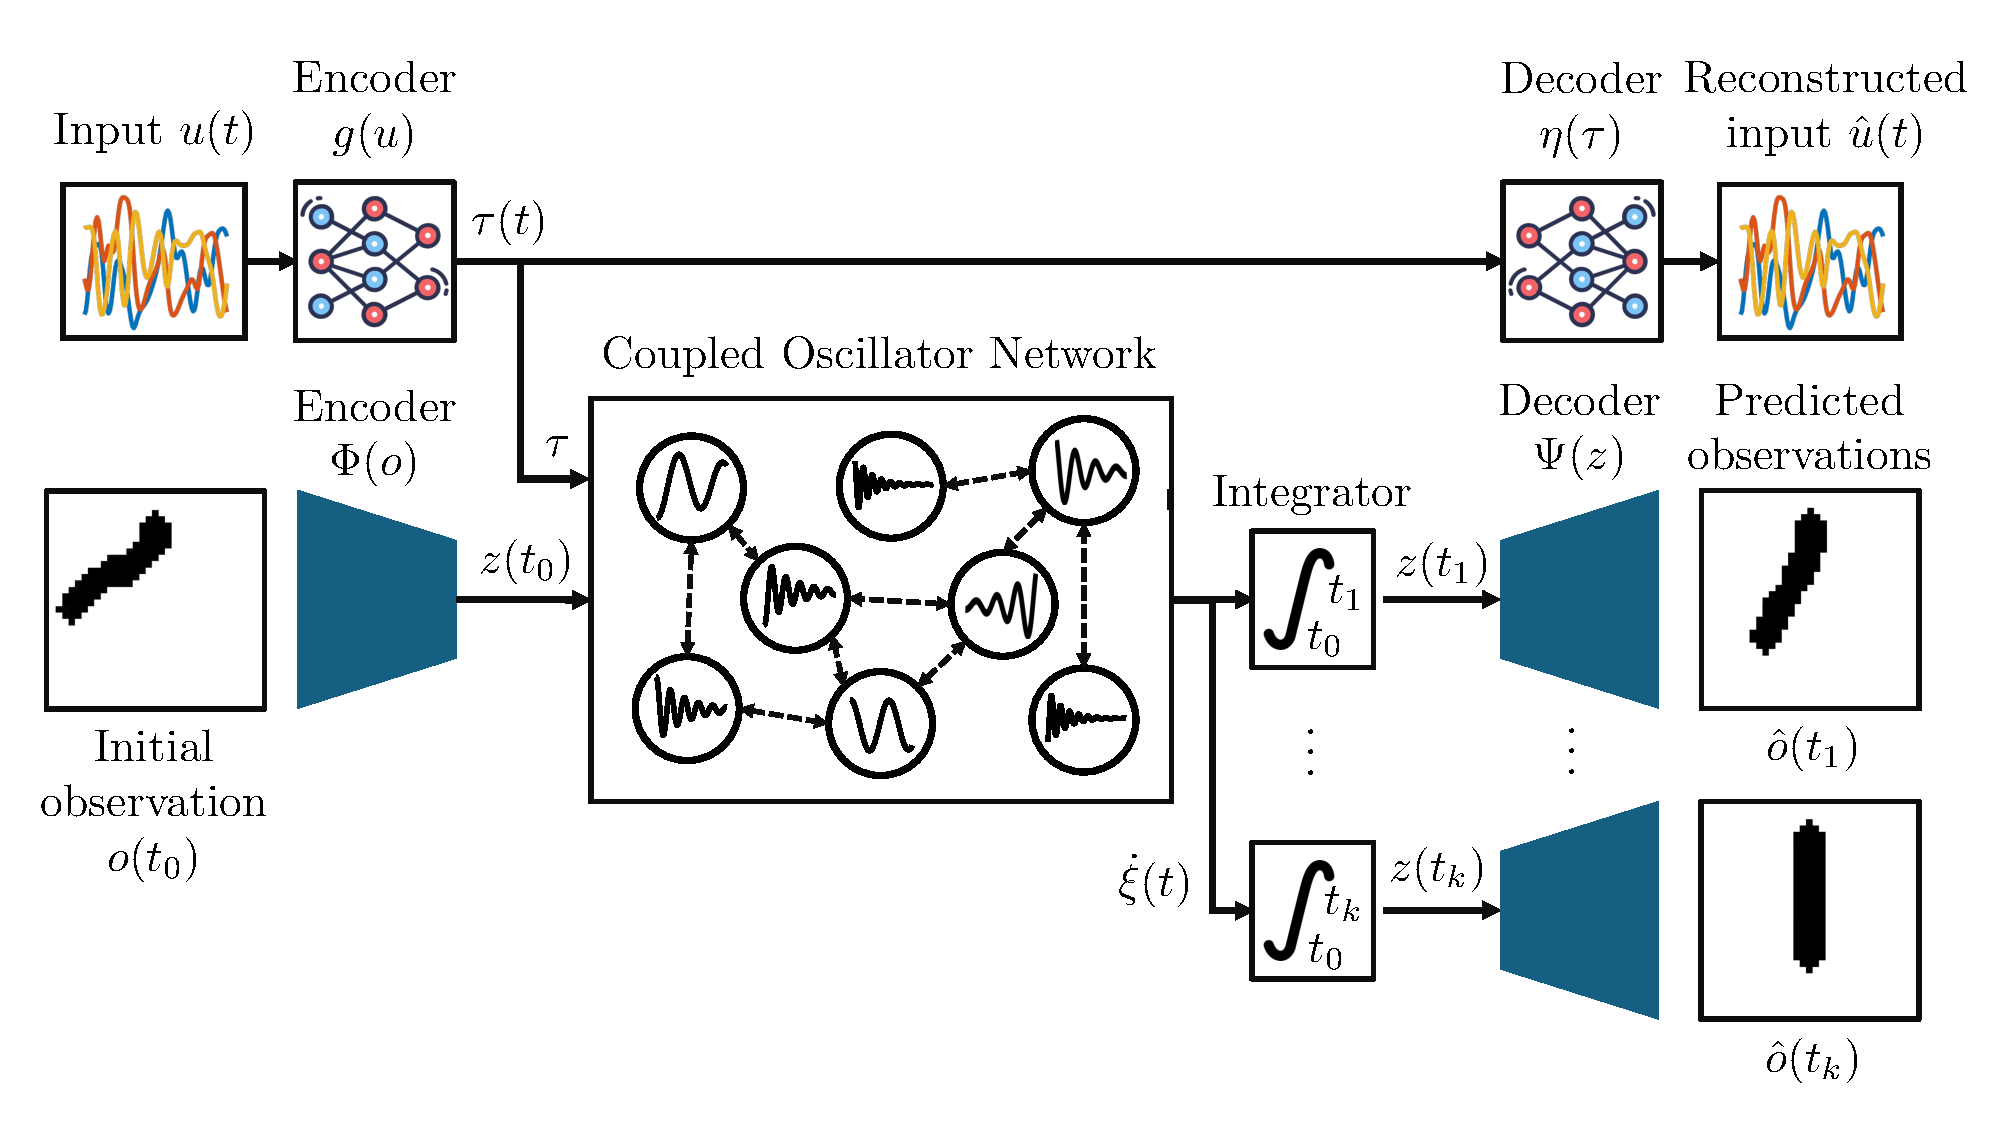
\includegraphics[width=1.0\columnwidth]{figures/autoencoder/blockdiagram_autoencoder_v1_cropped.pdf}
%     \caption{Exploiting \glspl{CON} for learning latent dynamics from pixels: We encode the initial observation $o(t_0)$ and the input $u(t)$ into latent space where we leverage the \gls{CON} to predict future latent states. Finally, we decode both the latent-space torques $\tau(t)$ and the predicted latent states $z(t)$.}
%     \label{fig:apx:blockdiagram_autoencoder}
% \end{figure}

When training the model, we jointly optimize $M_\mathrm{w}^{-1}, K_\mathrm{w}, D_\mathrm{w}, b$ and $g(u)$. 
However, we also need to make sure that we adhere to the stability constraints  $M_\mathrm{w}^{-1}, K_\mathrm{w}, D_\mathrm{w} \succ 0$. For this, we leverage the Cholvesky decomposition~\cite{petersen2008matrix}. Instead of directly learning the full matrix $A \in \mathbb{R}^{n_z \times n_z}$, we designate the elements of an upper triangular matrix $U \in \mathbb{R}^{n_z \times n_z}$ as the trainable parameters.
The Cholesky decomposition demands that $\mathrm{diag}(U_{11}, \dots, U_{n_z n_z}) > 0$. Therefore, we apply the operation
\begin{equation}
    U_{ii} = \log \left (1+ e^{\breve{U}_{ii} + \epsilon_1} \right ) + \epsilon_2,
\end{equation}
where $\breve{U}$ is the learned upper triangular matrix, and $\epsilon_1 = \num{1e-6}$ and $\epsilon_2 = \num{2e-6}$ are two small, positive values.
The positive-definite matrix $A$ is now given by $A = U^\mathrm{T} \, U \succ 0$.

\subsubsection{Neural ODEs}
We consider two kinds of Neural ODEs~\cite{chen2018neural}: the vanilla $f_\mathrm{NODE}: \xi(t) \times u(t) \mapsto \dot{\xi}(t)$ maps latent state and system actuation directly into a time derivative of the latent state. In contrast, for the \emph{MECH-NODE}, we enforce the latent dynamics to have a mechanical structure
\begin{equation}
    \dot{\xi}(t) = \begin{bmatrix}
        \frac{\mathrm{d} z}{\mathrm{d}t}\\
        \frac{\mathrm{d} \dot{z}}{\mathrm{d}t}
    \end{bmatrix} = \begin{bmatrix}
        \dot{z}(t)\\
        f_\mathrm{MECH-NODE}(\xi(t), u(t))
    \end{bmatrix}.
\end{equation}
We represent both $f_\mathrm{NODE}$ and $f_\mathrm{MECH-NODE}$ as \glspl{MLP} consisting of $5$ layers, a hidden dimension of $30$, and a hyperbolic tangent nonlinearity.

\subsubsection{Autoregressive models}

For the below stated autoregressive models, we divide the integration between two (latent) samples $\xi(t_k)$ and $\xi(t_{k+1})$ into $N_\mathrm{int}$ integration steps $\xi(t_k + \delta t), \dots, \xi(t_k + k' \delta t), \dots, \xi(t_k + N_\mathrm{int} \delta t)$ where $\delta t$ is the integration step size and $t_{k+1} = t_k + N_\mathrm{int} \delta t$. The autoregressive model now describes the transition $\xi(t_{k'+1}) = f_\mathrm{ar}(\xi(t_{k'}), u(t_k))) \: \forall k' \in 1, \dots, N_\mathrm{int}$.

\paragraph{RNN.}
We implement a standard, single-layer Elman RNN with \texttt{tanh} nonlinearity. The hidden state captures the latent state of the system. The latent state transition functions are given by
\begin{equation}
    \xi(t_{k'+1})
    % \begin{bmatrix}
    %     z(t_{k'+1})\\ \dot{z}(t_{k'+1})
    % \end{bmatrix}
    = \tanh(W_\mathrm{hh} \, \xi(t_{k'}) + b_\mathrm{hh} + W_\mathrm{ih} \, u(t_{k}) + b_\mathrm{ih}), 
\end{equation}
where $W_\mathrm{hh} \in \mathbb{R}^{2 n_z \times 2 n_z}$, $b_\mathrm{hh} \in \mathbb{R}^{2 n_z}$, $W_\mathrm{ih} \in \mathbb{R}^{2 n_z \times m}$, and $b_\mathrm{ih} \in \mathbb{R}^{2 n_z}$.

\paragraph{GRU.}
We implement a standard, single-layer GRU~\cite{cho2014learning} with \texttt{sigmoid} activation function where we interpret the latent state of the system as the hidden state of the cell. The latent state transition functions are given by
\begin{equation}
\begin{split}
    r =& \: \sigma \left ( W_\mathrm{hr} \, \xi(t_{k'}) + b_\mathrm{hr} + W_\mathrm{ir} \, u(t_{k}) + b_\mathrm{ir} \right )\\
    p =& \: \sigma \left ( W_\mathrm{hp} \, \xi(t_{k'}) + b_\mathrm{hp} + W_\mathrm{ip} \, u(t_{k}) + b_\mathrm{ip} \right )\\
    n =& \: \tanh \left ( r \odot \left ( W_\mathrm{hn} \, \xi(t_{k'}) + b_\mathrm{hn} \right) + W_\mathrm{in} \, u(t_{k}) + b_\mathrm{in} \right )\\
    \xi(t_{k'+1}) =& \: (1-p) \odot n + p \odot \xi(t_{k'})
\end{split}
\end{equation}
where $\sigma$ is the sigmoid function, $\odot$ the Hadamard product, $W_\mathrm{hr}, W_\mathrm{hp}, W_\mathrm{hn} \in \mathbb{R}^{2 n_z \times 2 n_z}$, $W_\mathrm{ir}, W_\mathrm{ip}, W_\mathrm{in} \in \mathbb{R}^{2 n_z \times m}$, and $b_\mathrm{hr}, b_\mathrm{ir}, b_\mathrm{ip}, b_\mathrm{in} \in \mathbb{R}^{2 n_z}$.

\paragraph{coRNN.} A time-discrete \gls{coRNN} is defined by the transition function
\begin{equation}
\begin{split}
    \xi(t_{k'+1}) = \begin{bmatrix}
        z(t_{k'+1})\\
        \dot{z}(t_{k'+1})
    \end{bmatrix} = \begin{bmatrix}
        z(t_{k'}) + \delta t \, \dot{z}(t_{k'})\\
        \dot{z}(t_{k'}) + \delta t \, \left ( - \gamma z(t_{k'}) - \varepsilon \dot{z}(t_{k'}) + \tanh \left ( W \xi(t_{k'}) + V u(t_k) + b \right ) \right )
    \end{bmatrix}
\end{split}
\end{equation}
where $\gamma, \varepsilon \in \mathbb{R}^+$ are positive, scalar hyperparameters representing the stiffness and damping coefficients, respectively. The term $\tanh \left ( W \xi(t_{k'}) + V u(t_k) + b \right )$ with $W \in \mathbb{R}^{2n_z \times 2n_z}$, $V \in \mathbb{R}^{n_z \times m}$, and $b \in \mathbb{R}^{n_z}$ contributes nonlinear state-to-state connections. It is implemented with a linear layer operating on $(\xi(t_{k'}), u(t_k))$ followed by a hyperbolic tangent nonlinearity.

\paragraph{CFA-CON.} We adapt the Alg.~\ref{alg:con:con_cfa} for predicting the time evolution in latent-space
\begin{equation}
    \xi(t_{k'+1}) = f_\mathrm{CFA-CON}(\xi(t_k'), u(t_k)),
\end{equation}
where $f_\mathrm{CFA-CON}$ describe the autoregressive state transition by the \gls{CFA-CON} model as introduced in Eq.~\ref{eq:con:cfa_con}.

\subsection{First-order variants of dynamical models}\label{sub:apx-con:1st_order_latent_dynamics}
For learning (latent) dynamics of \nth{1}-order systems (e.g., the reaction-diffusion dataset \emph{R-D}), it might be beneficial also to formulate the dynamical model to be of \nth{1}-order. 
While this is straightforward for some dynamics that do not explicitly take the order into account (e.g., RNN, GRU, NODE), for other models such as \gls{coRNN}, \gls{CON}, and \gls{CFA-CON} more adjustments are necessary.
Namely, we substitute the $\frac{\mathrm{d} z}{\mathrm{d}t}$ component of the \gls{ODE} with the expression for $\frac{\mathrm{d} \dot{z}}{\mathrm{d}t}$. Furthermore, we remove any terms that depend on the velocity $\dot{z}$ (e.g., damping effects).
Below, we report in detail the adapted, \nth{1}-order formulations for the \gls{coRNN}, \gls{CON}, and \gls{CFA-CON} models.

\paragraph{CON.} In the \nth{1}-order version, we adapt the standard, \nth{2}-order \gls{ODE} of the \gls{CON} network as defined in \eqref{eq:con:conw_dynamics} to
\begin{equation}
\begin{split}
    \dot{\xi}(t) = \dot{z}(t) = M_\mathrm{w}^{-1} \left ( g(u(t)) - K_\mathrm{w} z(t) - \tanh(z(t) + b) \right ).
\end{split}
\end{equation}

\paragraph{coRNN.} In the \nth{1}-order version, we define the transition function as
\begin{equation}
\begin{split}
    \xi(t_{k'+1}) = z(t_{k'+1}) = z(t_{k'}) - \delta t \, \gamma \, z(t_{k'}) + \delta t \, \tanh \left ( W \xi(t_{k'}) + V u(t_k) + b \right ).
\end{split}
\end{equation}

\paragraph{CFA-CON.}
We adapt a \nth{1}-order version of Alg.~\ref{alg:con:con_cfa} for predicting the time evolution in latent-space
\begin{equation}
\begin{split}
    \xi(t_{k'+1}) = z(t_{k'+1}) = z(t_{k'}) + \int_{t_{k'}}^{t_{k'} + \delta t} F(t_{k'}) - \kappa \, z(t')  \, \mathrm{d}t',\\
    F(t_{k'}) = g(u(t_{k})) - (K - \kappa) z(t_{k'}) - \tanh(W z(t_{k'}) + b),
\end{split}
\end{equation}
where the closed-form solution for the integral is given by
\begin{equation}
    \int_{t_{k'}}^{t_{k'} + \delta t} F(t_{k'}) - \kappa \, z(t')  \, \mathrm{d}t' = \frac{F(t_{k'})}{\kappa} \left ( 1 - \, e^{- \kappa \, \delta t} \right ).
\end{equation}

\subsection{Training}
We implement the network dynamics and the neural networks (e.g., encoder, decoder, and \glspl{MLP}) in JAX~\cite{jax2018github} and Flax~\cite{flax2020github}, respectively. When training or inferring time-continuous dynamical models (e.g., NeuralODE, CON), we rely on Diffrax~\cite{kidger2021neural} for numerical integration of the \gls{ODE} using the Dormand-Prince's 5/4 method~\cite{dormand1980family} (Dopri5). For the numerical integration of both the time-continuous and the time-discrete models (e.g., RNN, \gls{coRNN}, \gls{CFA-CON}), we use an integration time-step $\delta t$ of \SI{0.025}{s} and $\SI{0.01}{s}$ for the \emph{Toy Physics}~\cite{botev2021priors} and soft robotic datasets, respectively.

Because of the GPU memory constraints, we limit ourselves to a batch size of $30$ and $80$ trajectories for the \emph{Toy Physics}~\cite{botev2021priors} and soft robotic datasets, respectively.
We implement a learning rate schedule consisting of a warm-up (5 epochs) and a cosine annealing~\cite{loshchilov2016sgdr} period (remaining epochs). 
We employ an AdamW optimizer~\cite{kingma2014adam, loshchilov2018decoupled} with $\beta_1 = 0.9$, $\beta_2 = 0.999$ for updating both neural network weights (e.g., encoder, decoder) and parameters of the dynamical model (e.g., $K_\mathrm{}, D_\mathrm{w}$, $M_\mathrm{w}$, etc.).

\subsection{Evaluation metrics}
Similar to other publications in the field~\cite{liu2018image, yu2018generative, stolzle2022reconstructing}, % more citations about evaluation metrics: \cite{yi2020cosmovae, yang2017high}
we state the \gls{RMSE}, the \gls{PSNR} and the \gls{SSIM}~\cite{wang2004image} between the ground-truth image $o \in \mathbb{R}^{h_\mathrm{o} \times w_\mathrm{o}}$ and the predicted image image $\hat{o} \in \mathbb{R}^{h_\mathrm{o} \times w_\mathrm{o}}$.
We use the separated test set for all evaluation results.

\subsubsection{Root Mean-Square Error}
The \gls{RMSE} between the two images is given by
\begin{equation}
    \text{RMSE}(o, \hat{o}) = \sqrt{\sum_{u = 1}^{h_\mathrm{o}} \sum_{v = 1}^{w_\mathrm{o}} \frac{(o_{uv} - \hat{o}_{uv})^2}{h_\mathrm{o} \, w_\mathrm{o}}}.
\end{equation}

\subsubsection{Peak Signal-to-Noise Ratio}
The \gls{PSNR} is a function of the total \gls{MSE} loss and the maximum dynamic range of the image $L$. 
\begin{equation}
    \mathrm{PSNR}(o, \hat{o}) = 20 \, \log_{10} (L) - 10 \, \log_{10} \left (\sum_{u = 1}^{h_\mathrm{o}} \sum_{v = 1}^{w_\mathrm{o}} \frac{(o_{uv} - \hat{o}_{uv})^2}{h_\mathrm{o} \, w_\mathrm{o}} \right ).
\end{equation}
As we work with normalized images with pixels in the interval $[-1, 1]$, the dynamic range is $L = 2$.
% It is important to mention that the \gls{PSNR} is not linearly accumulated over mini-batches but rather computed as a function of the \gls{MSE} loss over the entire dataset.

\subsubsection{Structural Similarity Index Measure}
As simple pixel-by-pixel metrics such as \gls{RMSE} or \gls{PSNR} tend to average out any encountered errors, this could lead to a situation in which a significant reconstruction error in a part of the image is not seen in the \gls{RMSE} metric but has a huge impact on the visual appearance of the reconstruction. \gls{SSIM}~\cite{wang2004image} incorporates not just the \emph{absolute errors}, but also the strong inter-dependencies between pixels, especially when they are spatially close.
The \gls{SSIM} metric between two observations $o$ and $\hat{o}$ is given by
\begin{equation}
    \mathrm{SSIM}(o, \hat{o}) = l^\alpha(o, \hat{o}) \, c^\beta(o, \hat{o}) \, s^\gamma(o, \hat{o}),
\end{equation}
where
\begin{equation}
    l(o, \hat{o}) = \frac{2 \mu_o \mu_{\hat{o}} + C_1}{\mu_o^2 + \mu_{\hat{o}}^2 + C_1},
    \quad
    c(o, \hat{o}) = \frac{2 \sigma_o \sigma_{\hat{o}} + C_2}{\sigma_o^2 + \sigma_{\hat{o}}^2 + C_2},
    \quad 
    s(o, \hat{o}) = \frac{\sigma_{o\hat{o}} + C_3}{\sigma_o \sigma_{\hat{o}} + C_3}.
\end{equation}
We use the constants $C_1 = (k_1 L)^2$, $C_2 = (k_2 L)^2$ and $C_3 = C_2 / 2$, where $L$ signifies the dynamic range as previously used for the \gls{PSNR} metric,
and $k_1 = 0.01$ and $k_2 = 0.03$. The average $\mu$ and the variance $\sigma^2$ is computed with a Gaussian filter with a 1D kernel of size $11$ and sigma $1.5$.
We set the weight exponents $\alpha$, $\beta$, and $\gamma$ for the luminance, contrast, and structure comparisons all to one.
We rely on the PIX library~\cite{deepmind2020jax} for efficiently computing the \gls{SSIM} metric.

\subsection{Compute resources}\label{apx:sub:compute_resource}
% We train all models on a desktop workstation with a 12th-Gen i9 12900KF CPU with 16 cores, 64 GB of RAM, and an Nvidia GeForce RTX 3090 GPU with 24 GB of VRAM.

We trained the models on several desktop workstations for a total duration of roughly \SI{150}{h}.
In total, we relied on 10x RTX 3090/4090 GPUs, each with 24 GB of VRAM, training the models in parallel.
Each workstation contained between 64 and 128 GB of RAM, and we used roughly 100 GB of total storage. 
Training each model on one random seed took between \SI{45}{min} and \SI{4}{h} depending on the model type, the integration time constant, and the number of trainable parameters.
The hyperparameter tuning we conducted beforehand (only on one random seed) took roughly the same time and computational resources as generating the final results.

For the control experiments, we additionally used a laptop with a 16-core Intel Core i7-10870H CPU and 32 GB RAM. We did not need to use a GPU for evaluating the model during closed-loop control.
\newpage
\section{Appendix on Learning Latent Dynamics}\label{sec:apx-con:latent_dynamics_results}
We report the full set of quantitative results, including the additional evaluation metrics \gls{PSNR} and \gls{SSIM}, in Tables~\ref{tab:apx-con:latent_dynamics_results:cs} to \ref{tab:apx-con:latent_dynamics_results:r-d}. For \emph{PCC-NS-2} in Tab.~\ref{tab:apx-con:latent_dynamics_results:pcc_ns-2}, we additionally also recorded the training steps per second on an Nvidia RTX 3090 GPU with a batch size of $80$ (which leads to $8080$ images per batch).
We plot the results of a sweep across the latent dimensions for the additional evaluation metrics \gls{PSNR} and \gls{SSIM} in Fig.~\ref{fig:apx-con:latent_dynamics_sweep_pcc_ns-2}. Correspondingly, we visualize the number of trainable parameters of each model vs. the latent dimension in Fig.~\ref{fig:apx-con:num_trainable_params_vs_n_z}.
In Figs.~\ref{fig:apx-con:latent_dynamics:sequence_of_stills:s-p+f:rollout6}-~\ref{fig:apx-con:latent_dynamics:sequence_of_stills:pcc_ns-2:rollout2}, we present sequences of stills for the rollout of the trained \emph{CON}(-M) models on the various datasets. 

\begin{table}[ht]
    \centering
    \begin{small}
    \begin{tabular}{c c c c c}
         \toprule
         \textbf{Model} & \textbf{RMSE} $\downarrow$ & \textbf{PSNR} $\uparrow$ & \textbf{SSIM} $\uparrow$ & \textbf{\# Parameters} $\downarrow$ \\
         \midrule
         RNN & $0.2739 \pm 0.0057$ & $4.16 \pm 0.02$ & $0.6958 \pm 0.0122$ & $88$\\
         GRU~\citep{cho2014learning} & $0.0267 \pm 0.0033$ & $\mathbf{6.13 \pm 0.09}$ & $0.9861 \pm 0.0022$ & $248$\\
         coRNN~\citep{rusch2020coupled} & $\mathbf{0.0265 \pm 0.0002}$ & $\mathbf{6.13 \pm 0.01}$ & $\mathbf{0.9853 \pm 0.0006}$ & $40$\\
         NODE~\citep{chen2018neural} & $\mathbf{0.0264 \pm 0.0010}$ & $\mathbf{6.14 \pm 0.03}$ & $\mathbf{0.9858 \pm 0.0009}$ & $3368$\\
         MECH-NODE & $0.0328 \pm 0.0034$ & $5.99 \pm 0.07$ & $0.9821 \pm 0.0024$ & $3244$\\
         CON (our) & $0.0303 \pm 0.0053$ & $6.05 \pm 0.13$ & $0.9847 \pm 0.0027$ & $\mathbf{34}$\\
         CFA-CON (our) & $0.0313 \pm 0.0026$ & $6.02 \pm 0.06$ & $0.9843 \pm 0.0008$ & $\mathbf{34}$\\
         \bottomrule
    \end{tabular}
    \end{small}
    \vspace{0.5cm}
    \caption{Benchmarking of \gls{CON} and \gls{CFA-CON} at learning latent dynamics on the \textbf{\emph{M-SP+F} (mass-spring with friction) dataset}. For all models, a latent dimension of $n_z=4$ is chosen.
    % Therefore, the input mapping of CON/CFA-CON is a constant matrix and there is not difference w.r.t. input mapping capacity (e.g, \emph{CON-S} vs. \emph{CON-M}). 
    As this dataset does not consider any inputs, we remove all parameters in the RNN, GRU, coRNN, CON, and CFA-CON models related to the input mapping.
    \emph{MECH-NODE} is a \gls{NODE} with prior knowledge about the mechanical structure of the system (i.e., $\frac{\mathrm{d}x}{\mathrm{d}t} = \dot{x}$). We report the mean and standard deviation over three different random seeds and the number of parameters of each latent dynamics model.
    }
    \label{tab:apx-con:latent_dynamics_results:m_sp_f}
\end{table}

\begin{table}[ht]
    \centering
    \begin{small}
    \begin{tabular}{c c c c c}
         \toprule
         \textbf{Model} & \textbf{RMSE} $\downarrow$ & \textbf{PSNR} $\uparrow$ & \textbf{SSIM} $\uparrow$ & \textbf{\# Parameters} $\downarrow$ \\
         \midrule
         RNN & $0.2378 \pm 0.0352$ & $4.31 \pm 0.15$ & $0.7568 \pm 0.0350$ & $88$\\
         GRU~\citep{cho2014learning} & $0.1457 \pm 0.0078$ & $4.78 \pm 0.05$ & $0.9168 \pm 0.0093$ & $248$\\
         coRNN~\citep{rusch2020coupled} & $0.1333 \pm 0.0044$ & $4.86 \pm 0.03$ & $0.9194 \pm 0.0055$ & $40$\\
         NODE~\citep{chen2018neural} & $\mathbf{0.1260 \pm 0.0013}$ & $\mathbf{4.91 \pm 0.01}$ & $\mathbf{0.9379 \pm 0.0009}$ & $3368$\\
         MECH-NODE & $0.1650 \pm 0.0205$ & $4.67 \pm 0.12$ & $0.8985 \pm 0.0153$ & $3244$\\
         CON (our) & $0.1303 \pm 0.0064$ & $4.88 \pm 0.04$ & $0.9175 \pm 0.0095$ & $\mathbf{34}$\\
         CFA-CON (our) & $0.1352 \pm 0.0073$ & $4.85 \pm 0.05$ & $0.9133 \pm 0.0052$ & $\mathbf{34}$\\
         \bottomrule
    \end{tabular}
    \end{small}
    \vspace{0.5cm}
    \caption{Benchmarking of \gls{CON} and \gls{CFA-CON} at learning latent dynamics on the \textbf{\emph{S-P+F} (single pendulum with friction) dataset}. For all models, a latent dimension of $n_z=4$ is chosen. 
    % This dataset does not contain inputs. Therefore, the input mapping of CON/CFA-CON is a constant matrix and there is not difference w.r.t. input mapping capacity (e.g, \emph{CON-S} vs. \emph{CON-M}). 
    As this dataset does not consider any inputs, we remove all parameters in the RNN, GRU, coRNN, CON, and CFA-CON models related to the input mapping.
    \emph{MECH-NODE} is a \gls{NODE} with prior knowledge about the mechanical structure of the system (i.e., $\frac{\mathrm{d}x}{\mathrm{d}t} = \dot{x}$). We report the mean and standard deviation over three different random seeds and the number of parameters of each latent dynamics model.
    }
    \label{tab:apx-con:latent_dynamics_results:s_p_f}
\end{table}

\begin{table}[ht]
    \centering
    \begin{small}
    \begin{tabular}{c c c c c}
         \toprule
         \textbf{Model} & \textbf{RMSE} $\downarrow$ & \textbf{PSNR} $\uparrow$ & \textbf{SSIM} $\uparrow$ & \textbf{\# Parameters} $\downarrow$ \\
         \midrule
         RNN & $0.1694 \pm 0.0004$ & $4.631 \pm 0.002$ & $0.7082 \pm 0.0032$ & $672$\\
         GRU~\citep{cho2014learning} & $0.1329 \pm 0.0005$ & $4.858 \pm 0.003$ & $\mathbf{0.8340 \pm 0.0021}$ & $1968$\\
         coRNN~\citep{rusch2020coupled} & $0.1324 \pm 0.0016$ & $4.862 \pm 0.012$ & $0.8229 \pm 0.0039$ & $348$\\
         NODE~\citep{chen2018neural} & $0.1324 \pm 0.0024$ & $4.861 \pm 0.016$ & $0.8101 \pm 0.0024$ & $4404$\\
         MECH-NODE & $0.1710 \pm 0.0111$ & $4.624 \pm 0.063$ & $0.7170 \pm 0.0439$ & $4032$\\
         CON (our) & $0.1323 \pm 0.0018$ & $4.862 \pm 0.013$ & $0.8067 \pm 0.0038$ & $\mathbf{246}$\\
         CFA-CON (our) & $\mathbf{0.1307 \pm 0.0012}$ & $\mathbf{4.873 \pm 0.008}$ & $0.8147 \pm 0.0034$ & $\mathbf{246}$\\
         \bottomrule
    \end{tabular}
    \end{small}
    \vspace{0.5cm}
    \caption{Benchmarking of \gls{CON} and \gls{CFA-CON} at learning latent dynamics on the \textbf{\emph{D-P+F} (double pendulum with friction) dataset}. For all models, a latent dimension of $n_z=12$ is chosen. 
    % This dataset does not contain inputs. Therefore, the input mapping of CON/CFA-CON is a constant matrix and there is not difference w.r.t. input mapping capacity (e.g, \emph{CON-S} vs. \emph{CON-M}). 
    As this dataset do not consider any inputs, we remove all parameters in the RNN, GRU, coRNN, CON, and CFA-CON models related to the input mapping.
    \emph{MECH-NODE} is a \gls{NODE} with prior knowledge about the mechanical structure of the system (i.e., $\frac{\mathrm{d}x}{\mathrm{d}t} = \dot{x}$). We report the mean and standard deviation over three different random seeds and the number of parameters of each latent dynamics model.
    }
    \label{tab:apx-con:latent_dynamics_results:d_p_f}
\end{table}

\begin{table}[ht]
    \centering
    \begin{small}
    \begin{tabular}{c c c c c}
         \toprule
         \textbf{Model} & \textbf{RMSE} $\downarrow$ & \textbf{PSNR} $\uparrow$ & \textbf{SSIM} $\uparrow$ & \textbf{\# Parameters} $\downarrow$ \\
         \midrule
         RNN & $\mathbf{0.1011 \pm 0.0009}$ & $\mathbf{25.92 \pm 0.08}$ & $\mathbf{0.9777 \pm 0.0004}$ & $696$\\
         GRU~\citep{cho2014learning} & $0.1125 \pm 0.0100$ & $24.99 \pm 0.74$ & $0.9730 \pm 0.0040$ & $2040$\\
         coRNN~\citep{rusch2020coupled} & $0.2537 \pm 0.0018$ & $17.93 \pm 0.06$ & $0.8820 \pm 0.0024$ & $\mathbf{336}$\\
         NODE~\citep{chen2018neural} & $0.2415 \pm 0.0021$ & $18.36 \pm 0.08$ & $0.8946 \pm 0.0023$ & $4374$\\
         MECH-NODE & $0.2494 \pm 0.0028$ & $18.08 \pm 0.10$ & $0.8898 \pm 0.0016$ & $4002$\\
         CON-S (our) & $0.1993 \pm 0.0646$ & $20.03 \pm 2.44$ & $0.9218 \pm 0.0380$ & $1386$\\
         CON-M (our) & $0.1063 \pm 0.0027$ & $25.49 \pm 0.22$ & $0.9758 \pm 0.0011$ & $8568$\\
         CFA-CON (our) & $0.1462 \pm 0.0211$ & $22.72 \pm 1.17$ & $0.9573 \pm 0.0103$ & $8568$\\
         \bottomrule
    \end{tabular}
    \end{small}
    \vspace{0.5cm}
    \caption{Benchmarking of \gls{CON} and \gls{CFA-CON} at learning latent dynamics on the \textbf{\emph{CS} (soft robot with one constant strain segment) dataset}. For all models, a latent dimension of $n_z=12$ is chosen. \emph{CON-S} and \emph{CON-M} are small and medium-sized versions of the \gls{CON} model, respectively. \emph{MECH-NODE} is a \gls{NODE} with prior knowledge about the mechanical structure of the system (i.e., $\frac{\mathrm{d}x}{\mathrm{d}t} = \dot{x}$). We report the mean and standard deviation over three different random seeds and the number of parameters of each latent dynamics model.
}
    \label{tab:apx-con:latent_dynamics_results:cs}
\end{table}

\begin{table}[ht]
    \centering
    \begin{scriptsize}
    \setlength\tabcolsep{2.0pt}
    \begin{tabular}{c c c c c c c c}
         \toprule
         \textbf{Model} & \textbf{RMSE} $\downarrow$ & \textbf{PSNR} $\uparrow$ & \textbf{SSIM} $\uparrow$ & \textbf{\# Parameters} $\downarrow$ & $\mathbf{\frac{\text{Train. steps}}{\text{second}}}$ $\uparrow$ & \textbf{Inf. time} [ms] $\uparrow$\\
         \midrule
         RNN & $0.1373 \pm 0.0185$ & $23.27 \pm 1.10$ & $0.9643 \pm 0.0077$ & $320$ & $1.87$ & $02.6$\\
         GRU~\citep{cho2014learning} & $0.0951 \pm 0.0021$ & $\mathbf{26.45 \pm 0.19}$ & $0.9730 \pm 0.0040$ & $928$ & $1.83$ & $03.2$\\
         coRNN~\citep{rusch2020coupled} & $0.2504 \pm 0.0899$ & $18.05 \pm 2.66$ & $0.9814 \pm 0.0006$ & $\mathbf{152}$ & $\mathbf{1.89}$ & $02.7$\\
         NODE~\citep{chen2018neural} & $0.1867 \pm 0.0561$ & $20.60 \pm 2.28$ & $0.8774 \pm 0.0857$ & $3856$ & $0.79$ & $50.2$\\
         MECH-NODE & $0.1035 \pm 0.0012$ & $25.07 \pm 0.06$ & $0.9778 \pm 0.0004$ & $3062$ & $0.79$ & $50.3$\\
         CON-S (our) & $0.0996 \pm 0.0012$ & $26.05 \pm 0.11$ & $\mathbf{0.9792 \pm 0.0007}$ & $676$ & $0.78$ & $50.2$\\
         CON-M (our) & $0.1008 \pm 0.0006$ & $25.95 \pm 0.05$ & $0.9786 \pm 0.0003$ & $7048$ & $0.60$ & $60.1$\\
         CFA-CON (our) & $0.1124 \pm 0.0025$ & $25.01 \pm 0.19$ & $0.9734 \pm 0.0012$ & $7048$ & $1.12$ & $13.6$\\
         \bottomrule
    \end{tabular}
    \end{scriptsize}
    \vspace{0.5cm}
    \caption{Benchmarking of \gls{CON} and \gls{CFA-CON} at learning latent dynamics on the \textbf{\emph{PCC-NS-2} (soft robot with two constant curvature segments) dataset}. For all models, a latent dimension of $n_z=8$ is chosen. \emph{CON-S} and \emph{CON-M} are small and medium-sized versions of the \gls{CON} model, respectively. \emph{MECH-NODE} is a \gls{NODE} with prior knowledge about the mechanical structure of the system (i.e., $\frac{\mathrm{d}x}{\mathrm{d}t} = \dot{x}$). We report the mean and standard deviation over three different random seeds. Furthermore, we state the number of parameters of each latent dynamics model and the training steps per second on a Nvidia RTX 3090 GPU. Each batch contains $80$ trajectories and $8080$ images of resolution 32x32px in total. Finally, we report the inference time averaged over $5000$ runs for performing a rollout of \SI{2.02}{s} (while encoding and decoding all images along the trajectory) on an Nvidia RTX 3090 GPU with a batch size of $1$.
}
    \label{tab:apx-con:latent_dynamics_results:pcc_ns-2}
\end{table}

\begin{table}[ht]
    \centering
    \begin{small}
    \begin{tabular}{c c c c c}
         \toprule
         \textbf{Model} & \textbf{RMSE} $\downarrow$ & \textbf{PSNR} $\uparrow$ & \textbf{SSIM} $\uparrow$ & \textbf{\# Parameters} $\downarrow$ \\
         \midrule
         RNN & $0.2232 \pm 0.0075$ & $19.05 \pm 0.29$ & $0.8955 \pm 0.0083$ & $696$\\
         GRU~\citep{cho2014learning} & $0.2148 \pm 0.0196$ & $19.38 \pm 0.76$ & $0.9039 \pm 0.0223$ & $2040$\\
         coRNN~\citep{rusch2020coupled} & $0.2474 \pm 0.0018$ & $18.15 \pm 0.06$ & $0.8877 \pm 0.0011$ & $\mathbf{336}$\\
         NODE~\citep{chen2018neural} & $0.3373 \pm 0.0565$ & $15.46 \pm 1.34$ & $0.7432 \pm 0.0935$ & $4374$\\
         MECH-NODE & $0.1900 \pm 0.0024$ & $20.45 \pm 0.11$ & $0.9315 \pm 0.0011$ & $4002$\\
         CON-S (our) & $\mathbf{0.1792 \pm 0.0038}$ & $\mathbf{20.96 \pm 0.18}$ & $\mathbf{0.9392 \pm 0.0023}$ & $1386$\\
         CON-M (our) & $\mathbf{0.1785 \pm 0.0023}$ & $\mathbf{20.99 \pm 0.11}$ & $\mathbf{0.9395 \pm 0.0018}$ & $8568$\\
         CFA-CON (our) & $0.1803 \pm 0.0003$ & $20.90 \pm 0.01$ & $0.9366 \pm 0.0004$ & $8568$\\
         \bottomrule
    \end{tabular}
    \end{small}
    \vspace{0.5cm}
    \caption{Benchmarking of \gls{CON} and \gls{CFA-CON} at learning latent dynamics on the \textbf{\emph{PCC-NS-3} (soft robot with three constant curvature segments) dataset}. For all models, a latent dimension of $n_z=12$ is chosen. \emph{CON-S} and \emph{CON-M} are small and medium-sized versions of the \gls{CON} model, respectively. \emph{MECH-NODE} is a \gls{NODE} with prior knowledge about the mechanical structure of the system (i.e., $\frac{\mathrm{d}x}{\mathrm{d}t} = \dot{x}$). We report the mean and standard deviation over three different random seeds and the number of parameters of each latent dynamics model.
}
    \label{tab:apx-con:latent_dynamics_results:pcc_ns-3}
\end{table}

\begin{table}[ht]
    \centering
    \begin{small}
    \begin{tabular}{c c c c c}
         \toprule
         \textbf{Model} & \textbf{RMSE} $\downarrow$ & \textbf{PSNR} $\uparrow$ & \textbf{SSIM} $\uparrow$ & \textbf{\# Parameters} $\downarrow$ \\
         \midrule
         RNN & $0.3763 \pm 0.0374$ & $3.82 \pm 0.12$ & $0.4463 \pm 0.1358$ & $\mathbf{20}$\\
         GRU~\citep{cho2014learning} & $0.3232 \pm 0.0368$ & $\mathbf{3.99 \pm 0.13}$ & $0.6798 \pm 0.0949$ & $52$\\
         \nth{1}-order coRNN~\citep{rusch2020coupled} & $\mathbf{0.0741 \pm 0.0001}$ & $\mathbf{5.35 \pm 0.00}$ & $\mathbf{0.9724 \pm 0.0014}$ & $\mathbf{20}$\\
         NODE~\citep{chen2018neural} & $\mathbf{0.0738 \pm 0.0007}$ & $\mathbf{5.36 \pm 0.01}$ & $\mathbf{0.9683 \pm 0.0022}$ & $3064$\\
         CON (our) & $0.1110 \pm 0.0160$ & $5.03 \pm 0.12$ & $0.9372 \pm 0.0109$ & $24$\\
         CFA-CON (our) & $0.1068 \pm 0.0059$ & $5.05 \pm 0.05$ & $0.9418 \pm 0.0026$ & $24$\\
         \bottomrule
    \end{tabular}
    \end{small}
    \vspace{0.5cm}
    \caption{Benchmarking of \gls{CON} and \gls{CFA-CON} at learning latent dynamics on the \textbf{\emph{R-D} (reaction-diffusion) dataset}. For all models, a latent dimension of $n_z=4$ is chosen.
    % Therefore, the input mapping of CON/CFA-CON is a constant matrix and there is not difference w.r.t. input mapping capacity (e.g, \emph{CON-S} vs. \emph{CON-M}). 
    As this dataset does not consider inputs, we remove all parameters in the RNN, GRU, coRNN, CON, and CFA-CON models related to the input mapping.
    Also, as the \emph{reaction-diffusion} system is governed by \nth{1}-order \gls{PDE} dynamics, we use specialized, \nth{1}-order version of the \emph{CON}, \emph{CFA-CON}, and \emph{coRNN} dynamics.
    We report the mean and standard deviation over three different random seeds and the number of parameters of each latent dynamics model.
    }
    \label{tab:apx-con:latent_dynamics_results:r-d}
\end{table}



\begin{figure}[hb]
    \centering
    \subfigure[PSNR vs. latent dimension $n_z$]{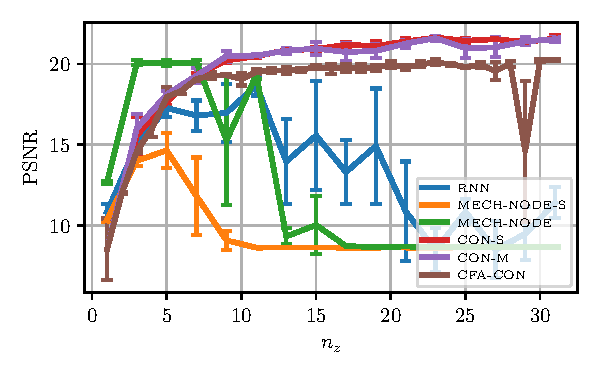
\includegraphics[width=0.49\textwidth, trim={5, 5, 5, 5}]{con/figures/results/latent_dynamics/pcc_ns-2/sweep_psnr_rec_dynamic_vs_n_z.pdf}}
    \subfigure[PSNR vs. model parameters]{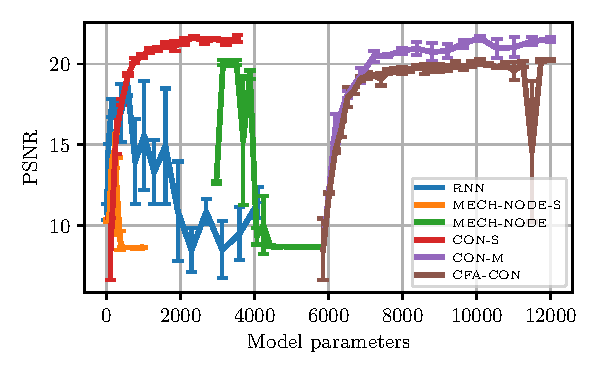
\includegraphics[width=0.49\textwidth, trim={5, 5, 5, 5}]{con/figures/results/latent_dynamics/pcc_ns-2/sweep_psnr_rec_dynamic_vs_num_trainable_params.pdf}}
    \\
    \subfigure[SSIM vs. latent dimension $n_z$]{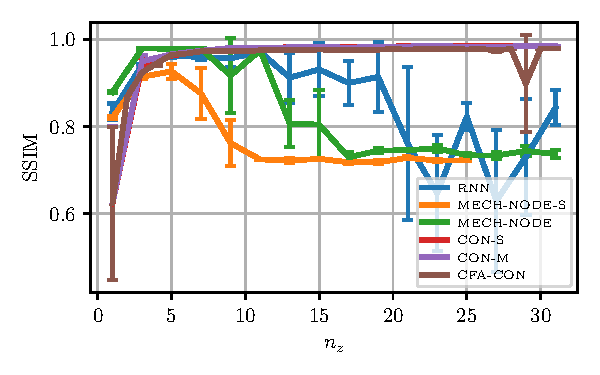
\includegraphics[width=0.49\textwidth, trim={5, 5, 5, 5}]{con/figures/results/latent_dynamics/pcc_ns-2/sweep_ssim_rec_dynamic_vs_n_z.pdf}}
    \subfigure[SSIM vs. model parameters]{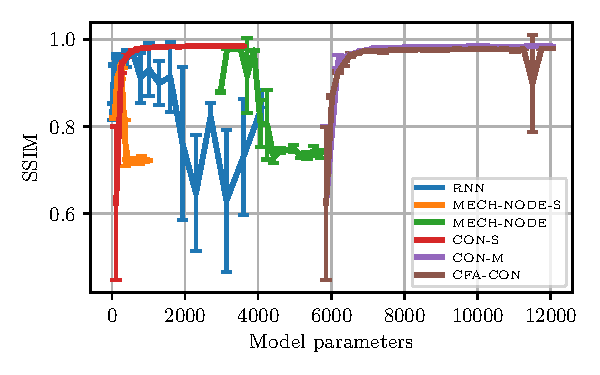
\includegraphics[width=0.49\textwidth, trim={5, 5, 5, 5}]{con/figures/results/latent_dynamics/pcc_ns-2/sweep_ssim_rec_dynamic_vs_num_trainable_params.pdf}}
    \caption{Evaluation of prediction performance of the various models vs. the dimension of their latent representation $n_z$ and the number of trainable parameters of the dynamics model, respectively. We optimize the hyperparameters for the case of $n_z=8$, and execute the tuning separately for each model and dataset.}
    \label{fig:apx-con:latent_dynamics_sweep_pcc_ns-2}
\end{figure}

\begin{figure}
    \centering
    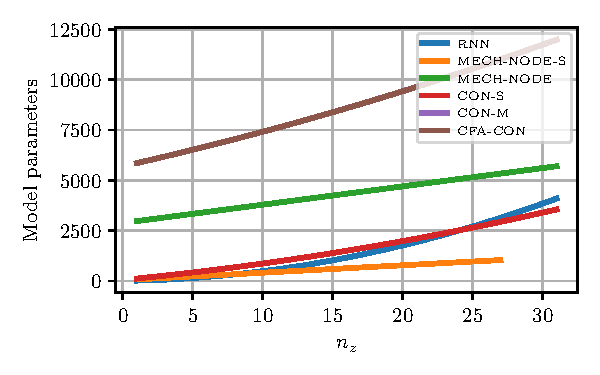
\includegraphics[width=0.6\columnwidth]{con/figures/results/latent_dynamics/pcc_ns-2/sweep_num_trainable_params_vs_n_z.pdf}
    \caption{Plot of number of trainable parameters vs. the latent dimension $n_z$ of various models trained on the \emph{PCC-NS-2} dataset. As we have configured them, \emph{CON-M} and \emph{CFA-CON} always have the same number of parameters (i.e., overlaying lines).}
    \label{fig:apx-con:num_trainable_params_vs_n_z}
\end{figure}

\begin{figure}[hb]
    \centering
    \subfigure{
\includegraphics[width=0.160\columnwidth]{con/figures/results/latent_dynamics/s-p+f/sequence_of_stills/rollout_6_target_0.00.png}}
    \subfigure{
\includegraphics[width=0.160\columnwidth]{con/figures/results/latent_dynamics/s-p+f/sequence_of_stills/rollout_6_target_0.55.png}}
    \subfigure{
\includegraphics[width=0.160\columnwidth]{con/figures/results/latent_dynamics/s-p+f/sequence_of_stills/rollout_6_target_1.10.png}}
    \subfigure{
\includegraphics[width=0.160\columnwidth]{con/figures/results/latent_dynamics/s-p+f/sequence_of_stills/rollout_6_target_1.65.png}}
    \subfigure{
\includegraphics[width=0.160\columnwidth]{con/figures/results/latent_dynamics/s-p+f/sequence_of_stills/rollout_6_target_2.20.png}}
    \subfigure{
\includegraphics[width=0.160\columnwidth]{con/figures/results/latent_dynamics/s-p+f/sequence_of_stills/rollout_6_target_2.75.png}}
    \\
    \setcounter{subfigure}{0}
    \subfigure[t=\SI{0.0}{s}]{
\includegraphics[width=0.160\columnwidth]{con/figures/results/latent_dynamics/s-p+f/sequence_of_stills/rollout_6_pred_0.00.png}}
    \subfigure[t=\SI{0.55}{s}]{
\includegraphics[width=0.160\columnwidth]{con/figures/results/latent_dynamics/s-p+f/sequence_of_stills/rollout_6_pred_0.55.png}}
    \subfigure[t=\SI{1.10}{s}]{
\includegraphics[width=0.160\columnwidth]{con/figures/results/latent_dynamics/s-p+f/sequence_of_stills/rollout_6_pred_1.10.png}}
    \subfigure[t=\SI{1.65}{s}]{
\includegraphics[width=0.160\columnwidth]{con/figures/results/latent_dynamics/s-p+f/sequence_of_stills/rollout_6_pred_1.65.png}}
    \subfigure[t=\SI{2.20}{s}]{
\includegraphics[width=0.160\columnwidth]{con/figures/results/latent_dynamics/s-p+f/sequence_of_stills/rollout_6_pred_2.20.png}}
    \subfigure[t=\SI{2.75}{s}]{
\includegraphics[width=0.160\columnwidth]{con/figures/results/latent_dynamics/s-p+f/sequence_of_stills/rollout_6_pred_2.75.png}}
    \caption{Prediction sequence of a \gls{CON} model with latent dimension $n_z=4$ trained on the single pendulum with friction (\emph{S-P+F}) dataset~\citep{botev2021priors}. 
    \textbf{Top row:} Ground-truth evolution of the system. \textbf{Bottom row:} Predictions of the \emph{CON} model. \newline
    The prediction model is given three images centered around $t=0$ for encoding the initial latent $z(0)$ and estimation of the initial latent velocity $\dot{z}(0)$. Subsequently, we roll out the autonomous network dynamics (i.e., unforced) and compare the decoded predictions with the ground-truth evolution of the system.  
    }\label{fig:apx-con:latent_dynamics:sequence_of_stills:s-p+f:rollout6}
\end{figure}

\begin{figure}[hb]
    \centering
    \subfigure{
\includegraphics[width=0.160\columnwidth]{con/figures/results/latent_dynamics/cs/sequence_of_stills/rollout_19_target_0.00.png}}
    \subfigure{
\includegraphics[width=0.160\columnwidth]{con/figures/results/latent_dynamics/cs/sequence_of_stills/rollout_19_target_0.04.png}}
    \subfigure{
\includegraphics[width=0.160\columnwidth]{con/figures/results/latent_dynamics/cs/sequence_of_stills/rollout_19_target_0.08.png}}
    \subfigure{
\includegraphics[width=0.160\columnwidth]{con/figures/results/latent_dynamics/cs/sequence_of_stills/rollout_19_target_0.12.png}}
    \subfigure{
\includegraphics[width=0.160\columnwidth]{con/figures/results/latent_dynamics/cs/sequence_of_stills/rollout_19_target_0.16.png}}
    \subfigure{
\includegraphics[width=0.160\columnwidth]{con/figures/results/latent_dynamics/cs/sequence_of_stills/rollout_19_target_0.20.png}}
    \\
    \setcounter{subfigure}{0}
    \subfigure[t=\SI{0.00}{s}]{
\includegraphics[width=0.160\columnwidth]{con/figures/results/latent_dynamics/cs/sequence_of_stills/rollout_19_pred_0.00.png}}
    \subfigure[t=\SI{0.04}{s}]{
\includegraphics[width=0.160\columnwidth]{con/figures/results/latent_dynamics/cs/sequence_of_stills/rollout_19_pred_0.04.png}}
    \subfigure[t=\SI{0.08}{s}]{
\includegraphics[width=0.160\columnwidth]{con/figures/results/latent_dynamics/cs/sequence_of_stills/rollout_19_pred_0.08.png}}
    \subfigure[t=\SI{0.12}{s}]{
\includegraphics[width=0.160\columnwidth]{con/figures/results/latent_dynamics/cs/sequence_of_stills/rollout_19_pred_0.12.png}}
    \subfigure[t=\SI{0.16}{s}]{
\includegraphics[width=0.160\columnwidth]{con/figures/results/latent_dynamics/cs/sequence_of_stills/rollout_19_pred_0.16.png}}
    \subfigure[t=\SI{0.20}{s}]{
\includegraphics[width=0.160\columnwidth]{con/figures/results/latent_dynamics/cs/sequence_of_stills/rollout_19_pred_0.20.png}}
    \caption{Prediction sequence of a forced \gls{CON} model with latent dimension $n_z=12$ trained on the soft robotic \emph{CS} dataset containing trajectories of a simulated constant strain robot with one segment. 
    \textbf{Top row:} Ground-truth evolution of the system. \textbf{Bottom row:} Predictions of the \emph{CON-M} model. \newline
    The prediction model is given three images centered around $t=0$ for encoding the initial latent $z(0)$ and estimation of the initial latent velocity $\dot{z}(0)$. Subsequently, we roll out the autonomous network dynamics (i.e., unforced) and compare the decoded predictions with the ground-truth evolution of the system.  
    }\label{fig:apx-con:latent_dynamics:sequence_of_stills:cs:rollout19}
\end{figure}


\begin{figure}[hb]
    \centering
    % image size: 575x575px
    \subfigure{
\includegraphics[width=0.192\columnwidth]{con/figures/results/latent_dynamics/pcc_ns-2/sequence_of_stills/rollout2-0001_gt.png}}
    \subfigure{
\includegraphics[width=0.192\columnwidth]{con/figures/results/latent_dynamics/pcc_ns-2/sequence_of_stills/rollout2-0002_gt.png}}
    \subfigure{
\includegraphics[width=0.192\columnwidth]{con/figures/results/latent_dynamics/pcc_ns-2/sequence_of_stills/rollout2-0003_gt.png}}
    \subfigure{
\includegraphics[width=0.192\columnwidth]{con/figures/results/latent_dynamics/pcc_ns-2/sequence_of_stills/rollout2-0004_gt.png}}
    \subfigure{
\includegraphics[width=0.192\columnwidth]{con/figures/results/latent_dynamics/pcc_ns-2/sequence_of_stills/rollout2-0005_gt.png}}
    \\
    \setcounter{subfigure}{0}
    \subfigure[t=\SI{0.0}{s}]{
\includegraphics[width=0.192\columnwidth]{con/figures/results/latent_dynamics/pcc_ns-2/sequence_of_stills/rollout2-0001_pred.png}}
    \subfigure[t=\SI{0.3}{s}]{
\includegraphics[width=0.192\columnwidth]{con/figures/results/latent_dynamics/pcc_ns-2/sequence_of_stills/rollout2-0002_pred.png}}
    \subfigure[t=\SI{0.6}{s}]{
\includegraphics[width=0.192\columnwidth]{con/figures/results/latent_dynamics/pcc_ns-2/sequence_of_stills/rollout2-0003_pred.png}}
    \subfigure[t=\SI{0.9}{s}]{
\includegraphics[width=0.192\columnwidth]{con/figures/results/latent_dynamics/pcc_ns-2/sequence_of_stills/rollout2-0004_pred.png}}
    \subfigure[t=\SI{1.2}{s}]{
\includegraphics[width=0.192\columnwidth]{con/figures/results/latent_dynamics/pcc_ns-2/sequence_of_stills/rollout2-0005_pred.png}}
    \caption{Prediction sequence of an unforced \gls{CON} model with latent dimension $n_z=8$ trained on the \emph{PCC-NS-2} dataset. 
    \textbf{Top row:} Ground-truth evolution of the system. \textbf{Bottom row:} Predictions of the \emph{CON-M} model. \newline
    The prediction model is given three images centered around $t=0$ for encoding the initial latent $z(0)$ and estimation of the initial latent velocity $\dot{z}(0)$. Subsequently, we roll out the autonomous network dynamics (i.e., unforced) and compare the decoded predictions with the ground-truth evolution of the system.  
    }\label{fig:apx-con:latent_dynamics:sequence_of_stills:pcc_ns-2:rollout2}
\end{figure}

\begin{figure}[hb]
    \centering
    % image size: 575x575px
    \subfigure{
\includegraphics[width=0.192\columnwidth]{con/figures/results/latent_dynamics/pcc_ns-2/sequence_of_stills/rollout1-0001_gt.png}}
    \subfigure{
\includegraphics[width=0.192\columnwidth]{con/figures/results/latent_dynamics/pcc_ns-2/sequence_of_stills/rollout1-0002_gt.png}}
    \subfigure{
\includegraphics[width=0.192\columnwidth]{con/figures/results/latent_dynamics/pcc_ns-2/sequence_of_stills/rollout1-0003_gt.png}}
    \subfigure{
\includegraphics[width=0.192\columnwidth]{con/figures/results/latent_dynamics/pcc_ns-2/sequence_of_stills/rollout1-0004_gt.png}}
    \subfigure{
\includegraphics[width=0.192\columnwidth]{con/figures/results/latent_dynamics/pcc_ns-2/sequence_of_stills/rollout1-0005_gt.png}}
    \\
    \setcounter{subfigure}{0}
    \subfigure[t=\SI{0.0}{s}]{
\includegraphics[width=0.192\columnwidth]{con/figures/results/latent_dynamics/pcc_ns-2/sequence_of_stills/rollout1-0001_pred.png}}
    \subfigure[t=\SI{0.3}{s}]{
\includegraphics[width=0.192\columnwidth]{con/figures/results/latent_dynamics/pcc_ns-2/sequence_of_stills/rollout1-0002_pred.png}}
    \subfigure[t=\SI{0.6}{s}]{
\includegraphics[width=0.192\columnwidth]{con/figures/results/latent_dynamics/pcc_ns-2/sequence_of_stills/rollout1-0003_pred.png}}
    \subfigure[t=\SI{0.9}{s}]{
\includegraphics[width=0.192\columnwidth]{con/figures/results/latent_dynamics/pcc_ns-2/sequence_of_stills/rollout1-0004_pred.png}}
    \subfigure[t=\SI{1.2}{s}]{
\includegraphics[width=0.192\columnwidth]{con/figures/results/latent_dynamics/pcc_ns-2/sequence_of_stills/rollout1-0005_pred.png}}
    \caption{Prediction sequence of a forced \gls{CON} model with latent dimension $n_z=8$ trained on the \emph{PCC-NS-2} dataset. 
    \textbf{Top row:} Ground-truth evolution of the system. \textbf{Bottom row:} Predictions of the \emph{CON-M} model. \newline
    The prediction model is given three images centered around $t=0$ for encoding the initial latent $z(0)$ and estimation of the initial latent velocity $\dot{z}(0)$. Subsequently, we provide the same constant input $u$ to both the simulator and the network dynamics (i.e., unforced) and compare the decoded predictions with the ground-truth evolution of the system.  
    }\label{fig:apx-con:latent_dynamics:sequence_of_stills:pcc_ns-2:rollout1}
\end{figure}
\newpage
\section{Appendix on Latent-space Control}\label{sec:apx-con:latent_space_control}
Below, we present supplementary results for the model-based, latent-space control on the two-segment, piecewise constant curvature soft robot (\emph{PCC-NS-2}).

\begin{figure}[ht]
    \centering
    \subfigure[Configuration $q(t) \in \mathbb{R}^2$]{\includegraphics[width=0.49\columnwidth, trim={5, 10, 5, 5}]{con/figures/results/control/pcc_ns-2/mech_node_psatid/setpoint_control_sequence_q.pdf}}
    \subfigure[Latent representation $z(t) \in \mathbb{R}^2$]{\includegraphics[width=0.49\columnwidth, trim={5, 10, 5, 5}]{con/figures/results/control/pcc_ns-2/mech_node_psatid/setpoint_control_sequence_z.pdf}}\\
    \subfigure[Control input $u(t) \in \mathbb{R}^2$]{\includegraphics[width=0.49\columnwidth, trim={5, 10, 5, 5}]{con/figures/results/control/pcc_ns-2/mech_node_psatid/setpoint_control_sequence_u.pdf}}
    \caption{Latent-space control of a continuum soft robot (simulated using two \gls{PCC} segments) following a sequence of setpoints with a pure \textbf{P-satI-D} feedback controller operating in a 2D latent space learned with the \textbf{MECH-NODE} model. The \gls{CON} model weights are initialized using a \textbf{random seed of 0}.
    The dotted and solid lines show the reference and actual values, respectively.
    For each setpoint, we randomly sample a desired shape $q^\mathrm{d}$ and render the corresponding image $o^\mathrm{d}$. This image is then encoded to a target latent $z^\mathrm{d}$. The controller then computes a latent-space torque $F^\mathrm{d}$, which is decoded to an input $u$. Finally, we provide this input to the simulator, which performs a roll-out of the closed-loop dynamics.
    Important: The robot's configuration (i.e., the first-principle, minimal-order state) is solely used for generating a target image and simulating the closed-loop system. 
    }\label{fig:apx-con:control:pcc_ns-2:mech_node_psatid_results}
\end{figure}


\begin{figure}[ht]
    \centering
    \subfigure[Configuration $q(t) \in \mathbb{R}^2$]{\includegraphics[width=0.49\columnwidth, trim={5, 10, 5, 5}]{con/figures/results/control/pcc_ns-2/con_psatid/setpoint_control_sequence_q.pdf}}
    \subfigure[Latent representation $z(t) \in \mathbb{R}^2$]{\includegraphics[width=0.49\columnwidth, trim={5, 10, 5, 5}]{con/figures/results/control/pcc_ns-2/con_psatid/setpoint_control_sequence_z.pdf}}\\
    \subfigure[Control input $u(t) \in \mathbb{R}^2$]{\includegraphics[width=0.49\columnwidth, trim={5, 10, 5, 5}]{con/figures/results/control/pcc_ns-2/con_psatid/setpoint_control_sequence_u.pdf}}
    \subfigure[Potential energy $U(t) \in \mathbb{R}$]{\includegraphics[width=0.49\columnwidth, trim={5, 10, 5, 5}]{con/figures/results/control/pcc_ns-2/con_psatid/setpoint_control_sequence_U.pdf}}
    \caption{Latent-space control of a continuum soft robot (simulated using two \gls{PCC} segments) following a sequence of setpoints with a pure \textbf{P-satI-D} feedback controller operating in a 2D latent space learned with the \textbf{\gls{CON}} model. The \gls{CON} model weights are initialized using a random seed of 0.
    The dotted and solid lines show the reference and actual values, respectively.
    For each setpoint, we randomly sample a desired shape $q^\mathrm{d}$ and render the corresponding image $o^\mathrm{d}$. This image is then encoded to a target latent $z^\mathrm{d}$. The controller then computes a latent-space torque $F^\mathrm{d}$, which is decoded to an input $u$. Finally, we provide this input to the simulator, which performs a roll-out of the closed-loop dynamics.
    Important: The robot's configuration (i.e., the first-principle, minimal-order state) is solely used for generating a target image and simulating the closed-loop system. 
    }\label{fig:apx-con:control:pcc_ns-2:con_PsatID_results}
\end{figure}


\begin{figure}[ht]
    \centering
    \subfigure[Configuration $q(t) \in \mathbb{R}^2$]{\includegraphics[width=0.49\columnwidth, trim={5, 10, 5, 5}]{con/figures/results/control/pcc_ns-2/con_psatid+ff/setpoint_control_sequence_q.pdf}}
    \subfigure[Latent representation $z(t) \in \mathbb{R}^2$]{\includegraphics[width=0.49\columnwidth, trim={5, 10, 5, 5}]{con/figures/results/control/pcc_ns-2/con_psatid+ff/setpoint_control_sequence_z.pdf}}\\
    \subfigure[Control input $u(t) \in \mathbb{R}^2$]{\includegraphics[width=0.49\columnwidth, trim={5, 10, 5, 5}]{con/figures/results/control/pcc_ns-2/con_psatid+ff/setpoint_control_sequence_u.pdf}}
    \subfigure[Potential energy $U(t) \in \mathbb{R}$]{\includegraphics[width=0.49\columnwidth, trim={5, 10, 5, 5}]{con/figures/results/control/pcc_ns-2/con_psatid+ff/setpoint_control_sequence_U.pdf}}
    \caption{Latent-space control of a continuum soft robot (simulated using two \gls{PCC} segments) following a sequence of setpoints with a pure \textbf{P-satI-D+FF} feedback \& feedforward controller operating in a 2D latent space learned with the \textbf{\gls{CON}} model. The \gls{CON} model weights are initialized using a random seed of 0.
    The dotted and solid lines show the reference and actual values, respectively.
    For each setpoint, we randomly sample a desired shape $q^\mathrm{d}$ and render the corresponding image $o^\mathrm{d}$. This image is then encoded to a target latent $z^\mathrm{d}$. The controller then computes a latent-space torque $F^\mathrm{d}$, which is decoded to an input $u$. Finally, we provide this input to the simulator, which performs a roll-out of the closed-loop dynamics.
    Important: The robot's configuration (i.e., the first-principle, minimal-order state) is solely used for generating a target image and simulating the closed-loop system. 
    }\label{fig:apx-con:control:pcc_ns-2:con_PsatID+FF_results}
\end{figure}

% \newpage
% \section{Extended Discussion on Future Applications and Limitations}\label{apx:sec:limitations}

\subsection{Systems for which we would expect the proposed method to work}
\paragraph{Mechanical systems with continuous dynamics, dissipation, and a single, attractive equilibrium point.}
The proposed method is a very good fit for mechanical systems with continuous dynamics, dissipation, and a single, attractive equilibrium point. In this case, the real system and the latent dynamics share the energetic structure and stability guarantees. Examples of such systems include many soft robots, deformable objects with dominant elastic behavior, and other mechanical structures with elasticity.

\paragraph{Local modeling of (mechanical) systems that do not meet the global assumptions.}
Even if the global assumptions of the proposed method are not met, the method can still be applied to model the local behavior around a local asymptotic equilibrium point of the system (i.e., in the case of multi-stability). For example, the method could be used to model the behavior of a robotic leg locally in contact with the ground, a cobot's interaction with its environment, etc.

\subsection{Systems for which we could envision the proposed method to work under (minor) modifications}
\paragraph{Mechanical systems without dissipation.}
The proposed method would currently not work well for mechanical systems without any dissipation, as (a) the original system will likely not have a globally asymptotically stable equilibrium point, and more importantly, (b) we currently force the damping learned in latent space to be positive definite. However, these systems are not common in practice as friction and other dissipation mechanisms are omnipresent, and the proposed method can learn very small damping values (e.g., the mass-spring+friction system). A possible remedy could be to relax the positive definiteness of the damping matrix in the latent space, allowing for zero damping. This would allow the method to work for systems without dissipation, such as conservative systems. Examples of such systems include a mass-spring system without damping, the n-body problem, etc.

\paragraph{Systems with discontinuous dynamics.}
The proposed method might underperform for systems with highly discontinuous dynamics, such as systems with impacts, friction, or other discontinuities. In these cases, the latent dynamics might not capture the real system's behavior accurately, and the control performance of feedforward + feedback will very likely be worse than pure feedback. Again, the method should be able to capture local behavior well. A possible remedy for learning global dynamics could be to augment the latent dynamics with additional terms that capture the discontinuities, such as contact and friction models (e.g., stick-slip friction).

\paragraph{Systems with multiple equilibrium points.}
The original system having multiple equilibria conflicts with the stability assumptions underlying the proposed CON latent dynamics. In this case, as, for example, seen on the pendulum+friction and double pendulum + friction results, the method might work locally but will not be able to capture the global behavior of the system. A possible remedy could be to relax the global stability assumptions of the CON network. For example, the latent dynamics could be learned in the original coordinates of CON while allowing $W$ also to be negative definite. This would allow the system to have multiple equilibria \& attractors. Examples of such systems include a robotic arm under gravity, pendula under gravity, etc.

\paragraph{Systems with periodic behavior.}
The proposed method will likely not work well for systems with periodic behavior, as they do not have a single, attractive equilibrium point. Examples of such systems include a mass-spring system with a periodic external force, a pendulum with a periodic external force, some chemical reactions, etc. Again, it is likely possible to apply the presented method to learning a local behavior (i.e., not completing the full orbit). A possible remedy could be to augment the latent dynamics with additional terms that capture the periodic behavior, such as substituting the harmonic oscillators with Van der Pol oscillators to establish a limit cycle or a supercritical Hopf bifurcation.

\subsection{Systems for which we would not expect the proposed method to work}
\paragraph{Nonholonomic systems.}
The proposed method likely would not work well for nonholonomic systems, as both structure (e.g., physical constraints) and stability characteristics would not be shared between the real system and the latent dynamics. Examples of such systems include vehicles, a ball rolling on a surface, and many mobile robots.

\paragraph{Partially observable and non-markovian systems.}
As the CON dynamics are evaluated based on the latent position and velocity encoded by the observation of the current time step and the observation-space velocity, we implicitly assume that the system is (a) fully observable and (b) fulfills the Markov property. This assumption might not hold for partially observable systems, such as systems with hidden states or systems with delayed observations. Examples of such cases include settings where the system is partially occluded or in situations without sufficient (camera) perspectives covering the system. Furthermore, time-dependent material properties, such as viscoelasticity or hysteresis, that are present and significant in some soft robots and deformable objects are not captured by the method in its current formulation.